\section{Tricks}

This section describes random tricks used to speed up rendering. They range from simple precomputed cos/sin tables to what I consider one of the most beautiful hacks in the engine: the Linear Feedback Shift Register.




\subsection{Cos/Sin Table Lookup}
\cw{cos} and \cw{sin} are expensive methods involving floating point calculations. They are extensively used at runtime. To speed things up, the engine generates and caches them in a lookup array (one value per angle) at startup. To save RAM, it exploits a math property ($cos(X) = sin(X + 90)$) to avoid 360 \cw{cos} method calls and 240 bytes of RAM by reusing the \cw{sin} table as follows:\\
\par
\label{cossintable}
\begin{minipage}{\textwidth}
\lstinputlisting[language=C]{code/sin_cos_table.c}
\end{minipage}


\begin{figure}[H]
 \centering
  \includegraphics[width=\textwidth]{imgs/drawings/cos_sin_table.pdf}
  \caption{In grey the 90 \cw{sin} values duplicated at the end of the array to complete the \cw{cos} lookup table.}
\end{figure}








\subsection{FizzleFade}
While most screen transitions are done with a fade to black (by shifting the palette), there are two instances when the screen transitions via fizzling:
\begin{itemize}
	\item When dying
	\item When killing a boss
\end{itemize}
Following on pages \pageref{fizzle1}, \pageref{fizzle2}, \pageref{fizzle3}, and \pageref{fizzle4} are a series of screenshots to illustrate fizzling.\\
\par
 During the transition, each pixel on the screen is turned to red (when dying) or blue (when dispatching a boss). Each pixel is written only once and seemingly at random. 



\begin{minipage}{\textwidth}
\centering \label{fizzle1}
  \scaledimage{.9}{fizzlefade/dying/screenshot_16.png}\\
  \vspace*{0.5cm}
  \scaledimage{.9}{fizzlefade/dying/screenshot_19.png}\\
\end{minipage}

\begin{minipage}{\textwidth}
\centering  \label{fizzle2}
  \scaledimage{.9}{fizzlefade/dying/screenshot_52.png} \\
  \vspace*{0.5cm}
  \scaledimage{.9}{fizzlefade/dying/screenshot_86.png} \\
\end{minipage}


\begin{minipage}{\textwidth}
\centering \label{fizzle3}
  \scaledimage{.9}{fizzlefade/boss/screenshot_60.png} \\
  \vspace*{0.5cm}
  \scaledimage{.9}{fizzlefade/boss/screenshot_66.png}  \\
\end{minipage}

\begin{minipage}{\textwidth}
\centering \label{fizzle4}
  \scaledimage{.9}{fizzlefade/boss/screenshot_102.png}\\
\vspace*{0.5cm}
  \scaledimage{.9}{fizzlefade/boss/screenshot_130.png}\\
\end{minipage}

To implement this effect, a naive approach would have been to use the pseudo random generator \cw{US\_RndT} and keep track of which pixels had been fizzled. However, this would make the fade non-deterministic with regard to duration and would also waste CPU cycles since the same pixel coordinates (X,Y) could come up several times. There is a faster and more elegant way to implement a pseudo-random value generator. The code responsible for this effect can be found in \cw{id\_vh.cpp}, in the function \cw{FizzleFade}. At first, it is not obvious how it works.\\
\par
\begin{minipage}{\textwidth}
\lstinputlisting[language=C]{code/fizzlefade.c}
\end{minipage}
\par
This code can be read as:\\
\begin{itemize}
\item Initialize \cw{rndval} to 1.
\item Break it down in 8 + 9 bits: use 8 bits to generate a Y coordinate and 9 bits for a X coordinate. Turn this pixel to red.
\item Subject \cw{rndval} to a soup of XORing.
\item When \cw{rndval} value is somehow back to 1: Stop.
\end{itemize}        
This feels like dark magic. How is \cw{rndval} supposed to return to value 1? Via a technique is called Linear Feedback Shift Register. The idea is to use one register to store a state, generate the next state, and also generate a value. To get the next value, you do a right shift. Since the rightmost bit disappears, a new one to the left is needed. To generate this new bit, the register uses "taps" which are bit offsets used to XOR together values and generate the new bit value. A Fibonacci representation shows a simple LFSR with two taps.\\
\par

\begin{figure}[H]
 \centering
  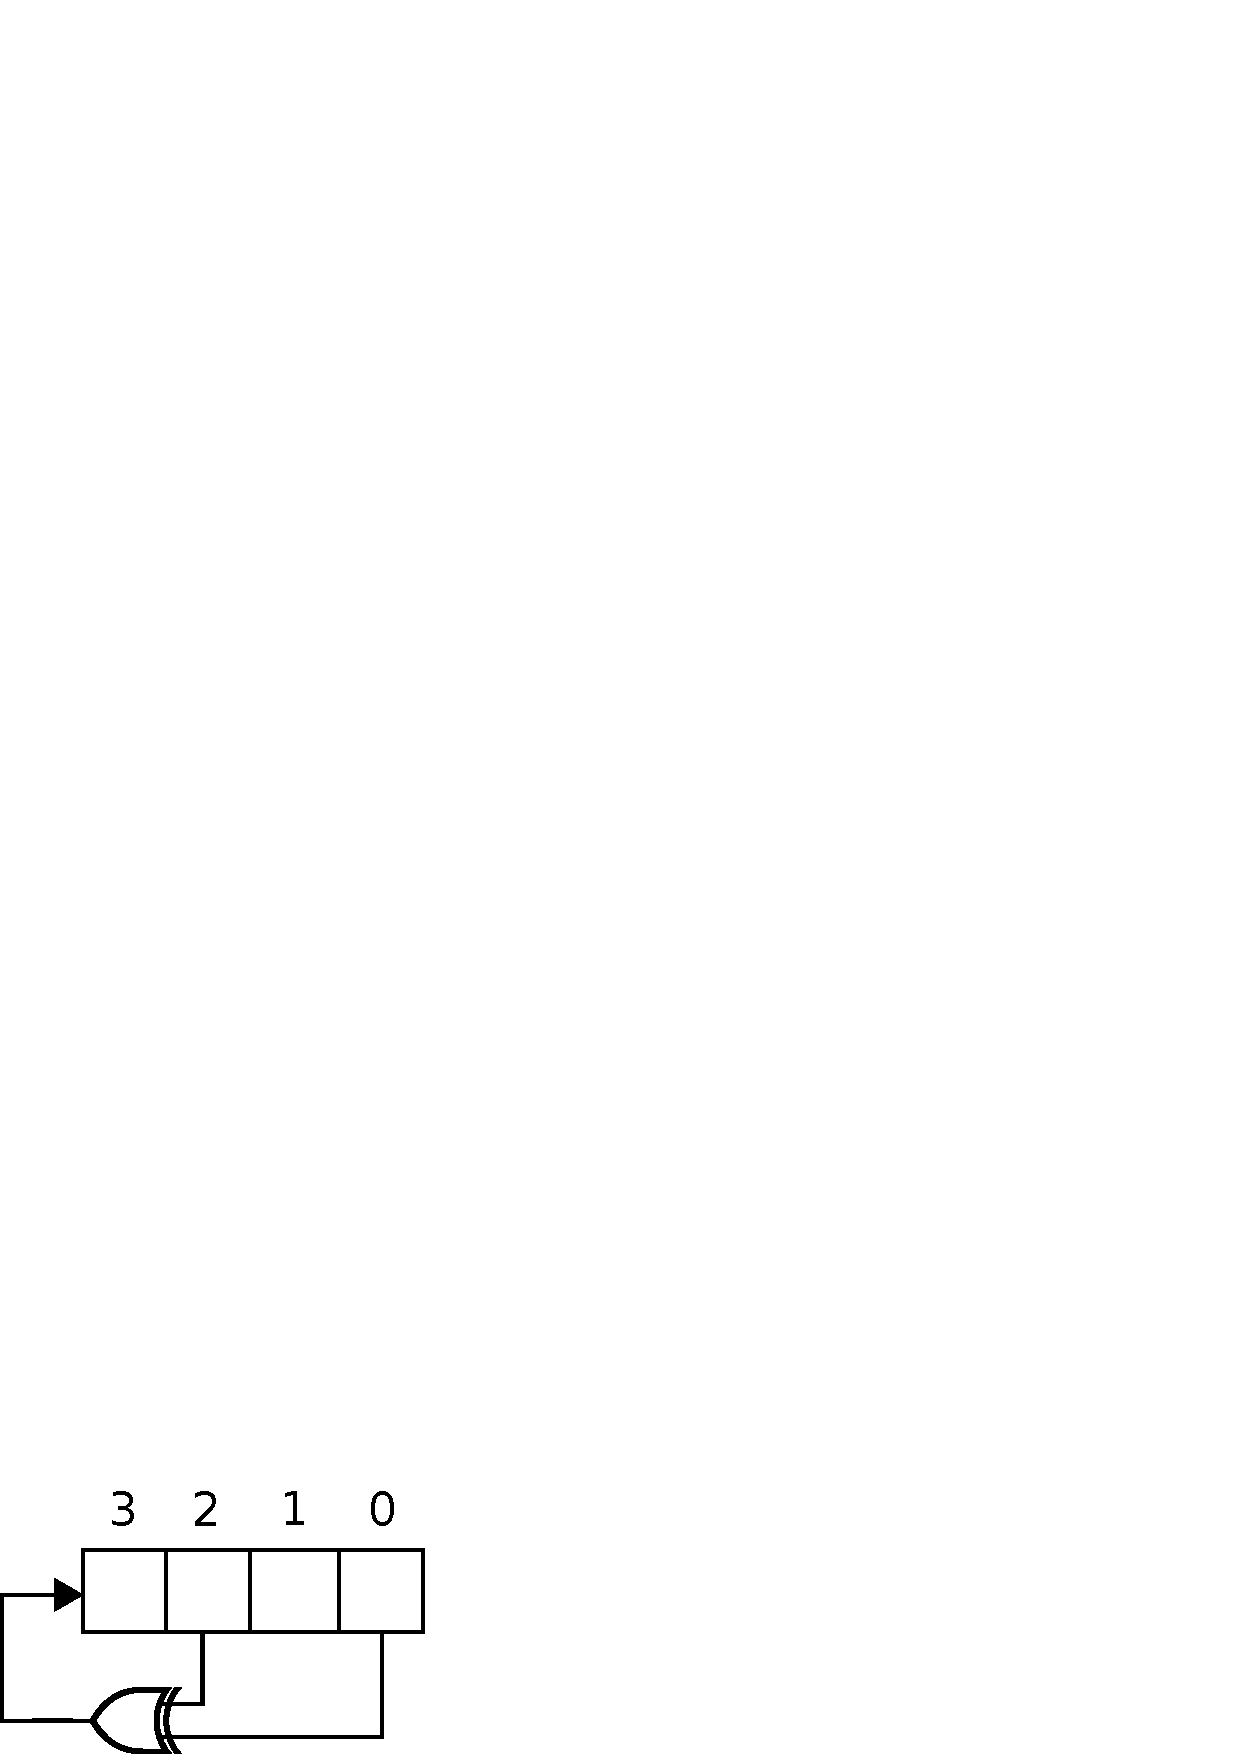
\includegraphics[width=.4\textwidth]{imgs/drawings/4bits_lfsr.pdf}
\end{figure}
The register depicted above is able to generate 6 values before it cycles back to its original state. The following listing shows all of them.\\
\par
\begin{minipage}{\textwidth}
\lstinputlisting{code/lfsr.txt}
\end{minipage}
\par
Various arrangements of taps will produce different series. In the case of this four bit register, the maximum number of values in a series is 16-1 = 15 (zero cannot be reached). This can be achieved with taps on bits 0 and 1. This is called a "Maximum-Length" LFSR.\\
\par
\begin{minipage}{\textwidth}
\lstinputlisting{code/maximum_lfsr.txt}
\end{minipage}
\par
\par
Wolfenstein 3D  uses a 17 bit Maximum-Length LFSR with two taps to generate a series of pseudo-random values. Of these 17 bits, on each iteration, 9 are used to generate a X coordinate and 8 for a Y coordinate. The corresponding pixel on screen is turned red/blue.\\
\par
\begin{figure}[H] 
   \centering \includegraphics[width=\textwidth]{imgs/drawings/fizzlefade/fibonacci.pdf} 
   \caption{17 bit Maximun-LFSR (Fibonacci representation).}
   \label{wolf_lfsr_fibo}
\end{figure}
\par
The Fibonacci representation helps to understand the general idea. But it is not how a LFSR is usually implemented in software. The reason is that it scales linearly with the number of taps. With four taps, you need three sequential XOR operations:
\par
\begin{figure}[H] 
    \centering 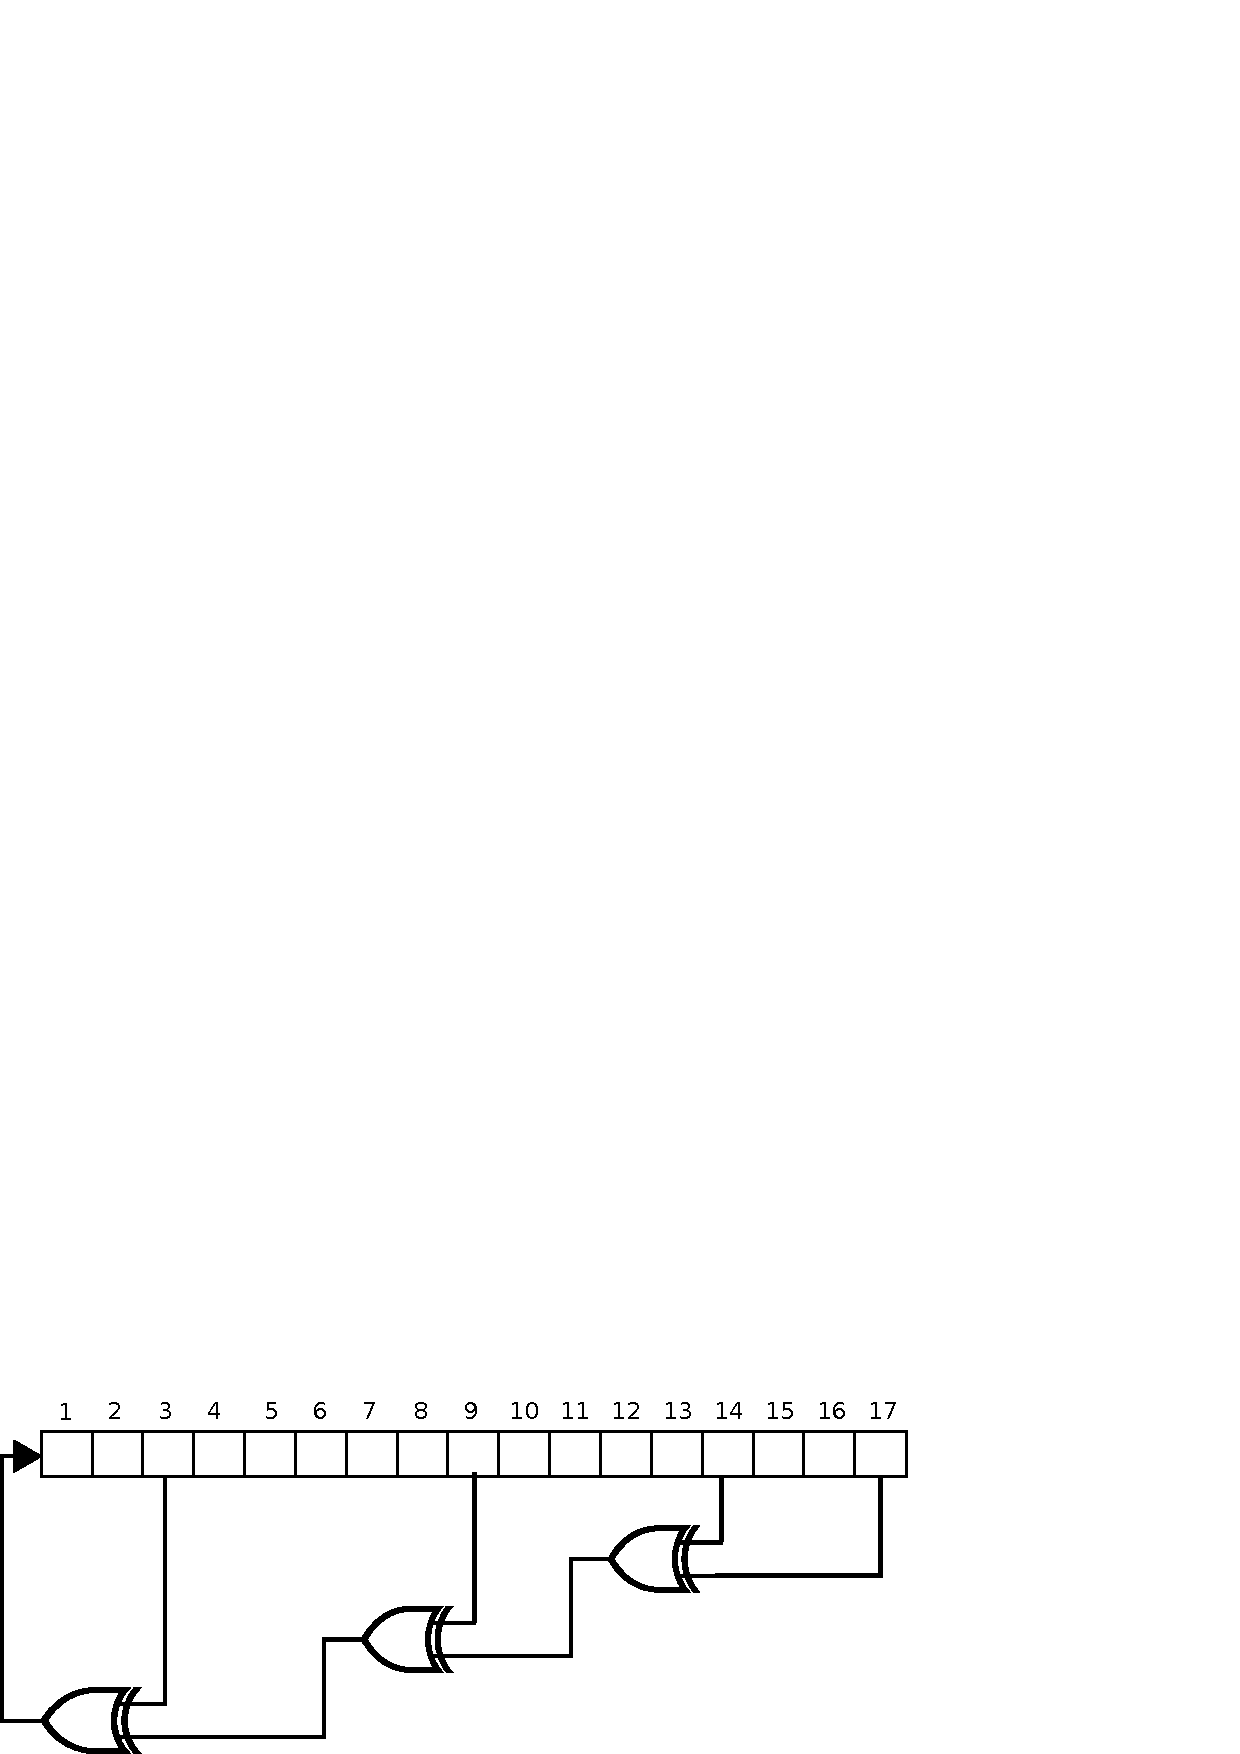
\includegraphics[width=\textwidth]{imgs/drawings/fizzlefade/fibonacci_hard.pdf} 
    \caption{Four taps on a 17 bit register; each XOR requires an instruction.}
\end{figure}
\par
There is an alternate way to represent a LFSR called "Galois", which allows one XOR operations regardless of how many taps are involved. It is the way Wolfenstein 3D implements its LFSR and writes 320x200=64000 pixels exactly once with a deterministic duration.
\par
\begin{figure}[H] 
    \centering 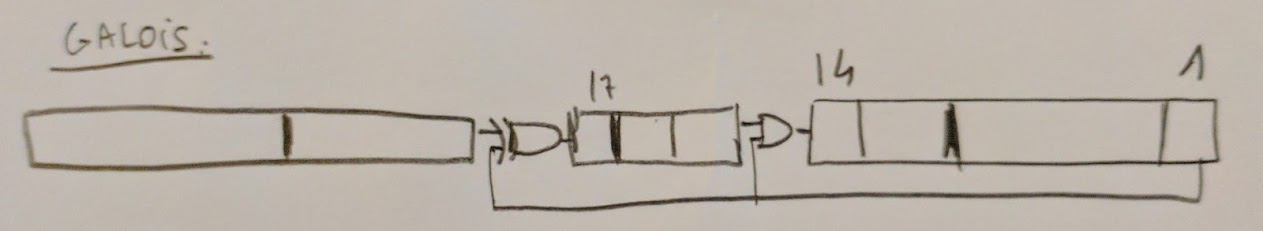
\includegraphics[width=\textwidth]{imgs/drawings/fizzlefade/galois.pdf} 
    \caption{Galois representation allows for one XOR operation regardless of the number of taps. This configuration is equivalent to figure \ref{wolf_lfsr_fibo}.}
\end{figure}
      
\bu{Note :} Because the effect works by plotting pixels individually, it was hard to replicate when developers tried to port the game to hardware accelerated GPU. None of the ports managed to replicate the fizzlefade except Wolf4SDL, which even found maximum-length LFSR taps configuration to reach resolution higher than 320x200.\\
\par
\bu{Note :} The tap configuration on 17 bits generates 131072 values before cycling. Since 320x200=64000, it could have been implemented with a 16 bit Maximum-length register with taps on 16,15,13 and 4 (in "Galois" notation).










\subsection{Palette}
Even though it limited the graphic capabilities of the game, the palette system can be turned into a strength. It is easy to fade the screen to white (when picking up an item), red (when taking damage), or black (when transitioning between 2D menus). It only takes 256*3 = 768 bytes and 768 out instructions to modify the full screen.
\begin{figure}[H]
  \centering
 \fullimage{palette_damage.png}
 \caption{The palette RGB colors is altered when taking damage.} \label{fig:palette_damage}
\end{figure}
A fast path is provided (which ironically only works if the CPU is as slow as the VGA processor) to update the palette via one \cw{rep outsb} instruction. Otherwise, if not supported, a loop of 768 \cw{outsb} is used.\\
\par
\begin{minipage}{\linewidth}
\lstinputlisting[language=C,morekeywords={asm,byte,far}]{code/vl_setpalette.c}
\end{minipage}








\section{Pseudo Random Generator}
Random numbers are necessary for many things during runtime, such as calculating whether an enemy is able to hit the player based on its accuracy. This is achieved with a precalculated pseudo-random series of 256 elements. The last random value is also the index of the next value.\\
\par
\begin{minipage}{\textwidth}
\lstinputlisting[language={[x86masm]Assembler}, style=mystyle,basicstyle=\small]{code/rndtable.asm}
\end{minipage}
\par
The pseudo-random series is initialized using the current time modulo 256 when the engine starts up.\\
\par

\begin{fancyquotes}
The random table wasn't even a shuffle - note that there are no 1s and two 2s in the table. I built it by just storing out 256 randoms from a little C program.  This was bad!
\bigskip \\
\textbf{John Carmack - Programmer}
 \end{fancyquotes}

\par
\begin{minipage}{\textwidth}
\lstinputlisting[language={[x86masm]Assembler}]{code/US_InitRndT.asm}
\end{minipage}
\par
The random number generator saves the last index in \cw{rndindex}. Upon request for a new number, it simply looks up the new value and updates \cw{rndindex}.
\par
\begin{minipage}{\textwidth}
\lstinputlisting[ language={[x86masm]Assembler}]{code/US_RndT.asm}
\end{minipage}

This pseudo random series of 256 values could have been generated with an 8 bit Maximum length LFSR (8,6,5,4). My assumption is that LFSR literature was hard to find at the time and finding the correct tap for a 16 bit maximum length register was not worth the effort.\\







